\def\ifundefined#1{\expandafter\ifx\csname#1\endcsname\relax} \ifundefined{preambleloaded}
\typeout{PRECOMILED PREAMBLE NOT LOADED}\documentclass[parskip=half, bibliography=totoc, captions=tableheading]{scrartcl} %Ich habe [parskip=half] hinzugefügt

%\usepackage[calc]{picture}
\usepackage{fixltx2e}

\usepackage{tcolorbox}

%\pagestyle{headings}
\usepackage[headtopline,headsepline]{scrpage2}
\setheadsepline{.5pt}
\pagestyle{scrheadings}
\cfoot[\pagemark]{\pagemark}
%\ihead{\headmark}
%\ihead{\headmark}
\ohead{16. Dezember 2016}
\automark{section}


\usepackage{polyglossia}
\setmainlanguage{german}
\usepackage{caption}
\usepackage{amsmath}
\usepackage{amssymb}
\usepackage{mathtools}

\usepackage{fontspec}
\defaultfontfeatures{Ligatures=TeX}

\usepackage[
  math-style=ISO,
  bold-style=ISO,
  sans-style=italic,
  nabla=upright,
]{unicode-math}

\setmathfont{Latin Modern Math}
%\setmathfont[range={\mathscr, \mathbfscr}]{XITS Math}
%\setmathfont[range=\coloneq]{XITS Math}
%\setmathfont[range=\propto]{XITS Math}

\usepackage[autostyle]{csquotes}

\usepackage[
  locale=DE,                   % deutsche Einstellungen
  separate-uncertainty=true,   % Immer Fehler mit \pm
  per-mode=symbol-or-fraction, % m/s im Text, sonst Brüche
]{siunitx}
%\sisetup{math-stylemicro=\text{µ},text-micro=µ}

\usepackage{xfrac}

\usepackage[section, below]{placeins}
\usepackage[
  labelfont=bf,
  font=small,
  width=0.9\textwidth,
]{caption}

\usepackage{subcaption}

\usepackage{graphicx}

\usepackage{float}
\floatplacement{figure}{h}
\floatplacement{table}{h}

\usepackage{booktabs}



\usepackage{bookmark}

\usepackage[shortcuts]{extdash}

\usepackage[math]{blindtext}

\usepackage{microtype}

\usepackage[
  backend=biber,
]{biblatex}
% Quellendatenbank
\addbibresource{lit.bib}

\usepackage{hyperref}

\usepackage{color} % Das ist Geschmacksfrage

\usepackage{makeidx} %Ich habe makeidx hinzugefügt + makeindex
\makeindex


\usepackage[version=3]{mhchem} % für Thermodynamik-chemische Elemente
\usepackage{enumitem} %Ich habe enumitem hinzugefügt
\usepackage{expl3}
\usepackage{xparse}
%\ExplSyntaxOn

\NewDocumentCommand \dif {m}
{
\mathinner{\symup{d} #1}
}
\usepackage{subcaption}


%\usepackage{showframe}
\author{Steven Becker \\
steven.becker@tu-dortmund.de \\
und \\
Stefan Grisard \\
stefan.grisard@tu-dortmund.de}

\title{Tutorium Experimentelle Physik I}
%\subtitle{}

\date{\today}
 \else
\typeout{\preambleloaded}
\fi

\begin{document}

\maketitle
\newpage

\setcounter{page}{1}
\section*{Zielsetzung}
Im Versuch 602 sollen Röntgenemissions- und Absorptionsspektren quantitativ untersucht werden.
Dies ermöglicht grundlegende Aussagen über den Atomaufbau und insbesondere die Energieniveaus
der betrachteten Stoffe.
\section{Theorie}
Als Röntgenstrahlung bezeichnet man elektromagnetische Strahlung im Energiebereich $\SI{10}{\kilo\eV}$
bis $\SI{100}{\kilo\eV}$. Röngenstrahlung befindet sich daher energetisch betrachtet zwischen oberhalb des sichtbaren Lichtes und
unterhalb von $\gamma$-Strahlung. Die hohe Energie ermöglicht eine Untersuchung von niedrigen Energieniveaus.
\subsection{Emission}
Zur Erzeugung von Röngenstrahlung wird eine Röntgenröhre nach Abbildung \ref{fig: röhre} verwendet. In einem
evakuierten Behälter werden aus einem Glühdraht Elektronen emittiert (Glühelektrischer Effekt) und durch eine
anliegende Spannung $U\ua{B}$ zu einer Kupferanode beschleunigt. Durch das Auftrefen an der Anode
entsteht die Röngenstrahlung. Hierbei setzt sich das entstehene Strahlungsspektrum aus zwei
Bestandteilen zusammen.\\
\begin{figure}
  \centering
  \includegraphics[width = 0.7\textwidth]{pics/röhre.png}
  \caption{Schematische Darstellung einer Röntgenröhre\cite{}.}
  \label{fig: röhre}
\end{figure}
Durch die Wechselwirkung mit dem Coulombfeld der Kerne des Anodenmaterials werden die Elektronen abgebremst. Da beschleunigte Ladungen strahlen, wird bei diesem
Vorgang ein Röntgenquant ausgesendet, dessen Energie $E\ua{ph} = h\nu$ genau dem Energieverlust des Elektrons
entspricht. Das hierdurch entstehende Spektrum ist kontinuierlich, da das Elektron auch nur Teile seiner
Energie verlieren kann. Die Maximale Energie der Photonen $E\ua{ph, max}$ wird dann erreicht,
wenn ein Elektron gänzlich abgebremst wird
\begin{equation}
  E\ua{ph, max} = \frac{h c}{\map{e}\ua{0}U\ua{B}}.
\end{equation}
Das sogenannte charakteristische Röntgenspektrum entsteht durch Ionisation des Anodenmaterials.
Wird ein Elektron aus einer der unteren Schalen ionisiert, rückt ein Elektron unter Aussendung eines
Photons, dessen Energie $E\ua{ph}$ genau der Energiedifferenz zwischen den Schalen entspricht, in die Fehlstelle nach.
\begin{equation}
  E\ua{ph} = h\nu = E\ua{m} - E\ua{n}.
\end{equation}
Die Ionisation kann nur dann stattfinden, wenn die Energie des Elektrons mindestens der Ionisationsenergie der betreffenden Schale entspricht.
Das Spektrum weist daher für das Anodenmaterial charakteristische diskrete Linien auf. Die Linien werden durch zwei Buchstaben
gekenntzeichnet. Der erste gibt die Schale ($K$, $L$, $M$ usw.) an, aus der ein Elektron ausgelöst wird, der zweite Buchstabe
($\alpha$, $\beta$ usw.) zeigt auf aus welcher höheren Schale ein Elektron nachgerückt. So kenntzeichnet etwa
$K\ua{\alpha}$ die Linie, die entsteht, wenn ein Elktron aus der $K$-Schale ionisiert wird und ein Elektron aus der $L$-Schale
nachrückt. Für die Bindungsenergien $E\ua{n}$ gilt
\begin{equation}
  E\ua{n} = -R\ua{\infty} z\ua{eff}^2 \frac{1}{n^2}.
\end{equation}
Hierbei entspricht $R\ua{\infty} = \SI{13.6}{\eV}$ der Rydbergenergie und $z\ua{eff}$ der effektiven Kernladung. Die effektive
Kernladung berücksichtigt die Abschirmung des Coulombpotentials in einem Mehrelektronenatom. Es gilt näherungsweise
\begin{equation}
  z\ua{eff} = z - \sigma\ua{n}.
\end{equation}
Mit der Kernladung $z$ und der Abschirmkonstante $\sigma\ua{n}$, deren Wert für alle Elektonen einer Schale als konstant angenommen wird.
Es ist zu beachten, dass die Elektronen eines Energieniveaus
aufgrund des individuellen Bahndrehimpulses bzw. Spins nicht alle die selbe Ionisierungsenergie besitzen. Daher besitzt das charakteristische
Spektrum eine Feinstruktur eng beianander liegender Linien.

\subsection{Absorption}
Die Absorption von Röntgenstrahlung wird im Wesentlichen durch den Photo- und den Compton-Effekt hervorgerufen. Die Absorption
fällt mit steigender Energie der Röntgenspannung. Bei diskreten Energien kommt es jedoch sprunghaft zu einem Anstieg. Diese
sogenannten Absorptionskanten treten genau bei den Ionisierungsenergien der Energieniveaus auf. Graphik \ref{fig: absorption} zeigt einen charakteristischen
Verlauf der Absorption unter variabler Wellenlänge ($E \propto \frac{1}{\lambda}$) der einfallenden Strahlung.
Die Absorptionskanten werden entsprechend der Schale bezeichnet, die ionisiert wird.
Auch hier ist die Feinstruktur zu beachten, die dazu
führt, dass für Schalen mit mehr als einem Elektron mehrere Kanten zu beobachten sind (z.B. $L\ua{I}$, $L\ua{II}$, $L\ua{III}$).
\begin{figure}[H]
  \centering
  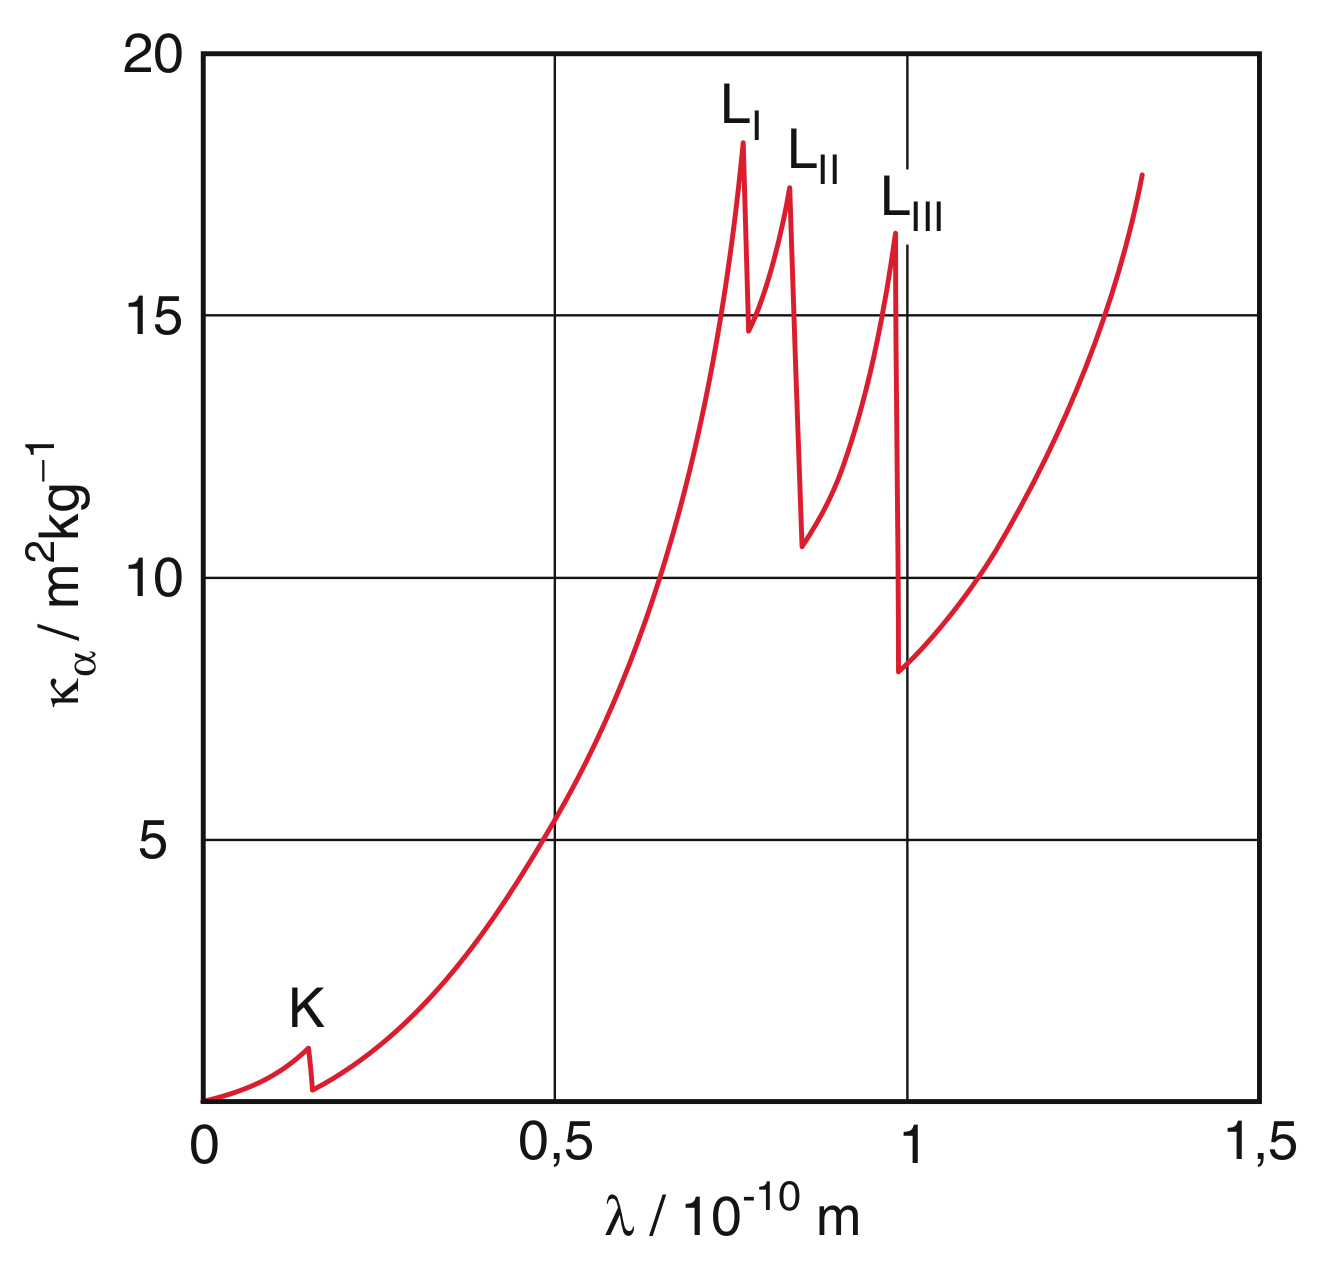
\includegraphics[width = 0.4\textwidth]{pics/absorption.png}
  \caption{Charakteristisches Röntgenabsorptionsspektrum für Blei\cite{}.}
  \label{fig: absorption}
\end{figure}

\subsection{Bragg-Bedingung}
Zur Analyse des Röntgenenergiespektrums wird ausgenutzt, dass die Beugung elektromagnetischerstrahlung an christallinen
Oberflächen von der Wellenlänge abhängt. Für die erste Beugungsordnung gilt nach der Bragg-Bedingung
\begin{equation}
  2 d \sin\theta = \lambda.
\end{equation}
Hierbei entspricht $d$ der Gitterkonstanten und $\theta$ dem Glanzwinkel.

\section{Versuchsaufbau/-durchführung}\label{abs: aufbau}
In diesem Abschnitt werden die verwendeten Brückenschaltungen aufgeführt. Als Quelle für
die Speisespannung wurde in allen Versuchteilen ein Wechselstromgenerator mit variabler Frequenz
verwendet. \\
Zur Bestimmung eines unbekannten ohmschen Widerstandes, wird die Wheatonsche Brücke
benutzt (Abbildung \ref{fig: wheaton}).
Der Zusammenhang \eqref{eq: widerstandsbedingungen} vereinfacht sich in diesem Fall zu:
\begin{equation}
  R_{\symup{X}} = R_2 \frac{R_3}{R_4}
\end{equation}
Das Verhältnis $R_3 / R_4$ ist durch ein Potentiometer realisiert. Um eine Fehlerrechnung durchführen
zu können, wird der Widerstand $R_2$ drei mal varriert und jeweils die entsprechenden Werte für $R_3$, die
zum Verschwinden der Brückenspannung führen, aufgenommen. Als Nullindikator wird ein Oszilloskop verwendet. \\
Nach dem selben Prinzip werden die Kapazität eines Kondensators und dessen Wirkwiderstand bestimmt. Der Aufbau
der Kapazitätsmessbrücke ist in Abbildung \ref{fig: kapazität} dargestellt.

\begin{figure}
\centering
\begin{subfigure}{0.49\textwidth}
  \centering
  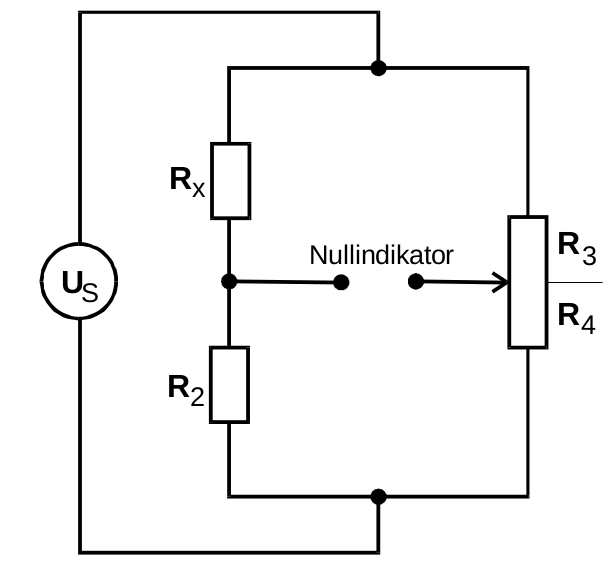
\includegraphics[width = 6cm]{pics/wheaton.png}
  \caption{Wheatonsche Brückenschaltung}
  \label{fig: wheaton}
\end{subfigure}
\begin{subfigure}{0.49\textwidth}
\centering
\includegraphics[width = 5.5cm]{pics/kap_brücke.png}
\caption{Kapazitätsmessbrücke}
\label{fig: kapazität}
\end{subfigure}
\caption{Wheaton- und Kapazitätsmessbrücke \cite{anleitung302}}
\label{fig: kapind}
\end{figure}

\begin{figure}
\centering
\begin{subfigure}{0.49\textwidth}
\centering
  \includegraphics[width = 4.6cm]{pics/ind_brücke.png}
\caption{Induktivitätsmessbrücke}
\label{fig: induktivität}
\end{subfigure}
\begin{subfigure}{0.49\textwidth}
  \centering
  \includegraphics[width = 6.8cm]{pics/max_brücke.png}
  \caption{Maxwell-Brücke}
  \label{fig: maxwell}
\end{subfigure}
\caption{Induktivitäts- und Maxwellmessbrücke\cite{anleitung302}}
\label{fig: indmax}
\end{figure}

Hierbei wird zunächst von einem idealen Kondensator ausgegangen, $R_x$ bzw. $R_2$ also aus der Schaltung entfernt. Für die
Kapazität $C_{\symup{X}}$ gilt in diesem Fall:
\begin{equation}
  C_{\symup{X}} = C_2 \frac{R_4}{R_3}
  \label{eq: Cx}
\end{equation}
Zur Bestimmung von $R_{\symup{X}}$ einer realen Kapazität wird als weiteres Stellglied der variable Widerstand $R_2$ in Reihe mit dem Kondesator $C_2$
geschaltet. Als weitere Bedingung für die Nullmethode neben \eqref{eq: Cx} ergibt sich:
\begin{equation}
  R_{\symup{X}} = R_2\frac{R_3}{R_4}
  \label{eq: Rx}
\end{equation}
Die Messung einer realen Induktivität wird zunächst mit einem Aufbau der Form \ref{fig: induktivität} durchgeführt.
Für $U_{\symup{Br}} = 0$ gelten hier die Bedingungen:
\begin{align}
  \begin{aligned}
    R_{\symup{X}} &= R_2\frac{R_3}{R_4} \\
    L_{\symup{X}} &= L_2\frac{R_3}{R_4}
  \end{aligned}
  \label{eq: Lx}
\end{align}

Anschließend geschieht die Induktivitätsmessung erneut mittels einer Maxwell-Brücke (siehe Abbildung \ref{fig: maxwell}).
Hierbei sind nun die Wiederstände $R_3$ und $R_4$ als unabhängige Stellglieder eingebaut. Die Bedingungen für die abgeglichene Brücke lauten
bei diesem Aufbau:
\begin{align}
  \begin{aligned}
    R_{\symup{X}} &=\frac{R_2 R_3}{R_4} \\
    L_{\symup{X}} &= R_2 R_3 C_4
  \end{aligned}
  \label{eq: Lx_maxwell}
\end{align}
Abschließend wird die Frequenzabhängigkeit einer Wien-Robinson-Brücke untersucht. Der Aufbau ist in Abbildung
 \ref{fig: wienrob} illustriert.
\begin{figure}
  \centering
  \includegraphics[width = 6cm]{pics/wien_rob_brücke.png}
  \caption{Wien-Robinson-Brücke\cite{anleitung302}}
  \label{fig: wienrob}
\end{figure}
Für das Verhältnis zwischen den Betragsquadraten der Speise- und Brückenspannung gilt:
\begin{equation}
  \left| \frac{\textfrak{U}_{\symup{Br}}}{\textfrak{U}_{\symup{S}}}\right|^2 = \frac{1}{9} \frac{(\Omega^2 - 1)^2 }{(1 - \Omega ^2)^2 + 9 \Omega ^2}
\end{equation}
Mit $\Omega = \frac{\omega}{\omega_0} = \omega R C$. Hierbei entspricht $\omega_0$ also der zu $\nu_0$ gehörigen Kreisfrequenz (siehe Abs. \ref{abs: theo}), die
für ein Verschwinden der Brückenspannung sorgt. Für variable Frequenzen $\nu \in [20, \num{30000}]\,\si{\hertz}$ werden $U_{\symup{S}}$ bzw. $U_{\symup{Br}}$ mit einem
Voltmeter bzw. der Peak-to-Peak-Einstellung des Oszilloskops gemessen. Die Untersuchung der Frequenzabhängigkeit
 ermöglicht in der Auswertung die Berechnung des Klirrfaktors \eqref{eq: klirr}.

\section{Auswertung}

Die in der Auswertung bestimmten Ausgleichsrechnungen werden mit
der Funktion \emph{curve\_ fit} \cite{scipy} aus dem Python Paket \emph{scipy.optimize}\cite{scipy} durchgeführt.

\subsection{Auswertung der $T_{00}$ Mode}
\FloatBarrier
In der Tabelle \ref{tab: T_00} befinden sich die aufgenommenen Messwerte.
\begin{table} 
\centering 
\caption{Messwerte der T_00 Mode.} 
\label{tab: T_00} 
\begin{tabular}{S S } 
\toprule  
{$r / \si{ \milli\meter }$} & {$I_p / \si{ \micrompere}$} \\ 
\midrule  
-10.0 & 2.2\\ 
-9.0 & 3.1\\ 
-8.0 & 3.9\\ 
-7.0 & 5.0\\ 
-6.0 & 6.2\\ 
-5.0 & 7.4\\ 
-4.0 & 8.4\\ 
-3.0 & 9.4\\ 
-2.0 & 9.4\\ 
-1.0 & 9.2\\ 
0.0 & 8.8\\ 
1.0 & 8.1\\ 
2.0 & 7.2\\ 
3.0 & 6.1\\ 
4.0 & 5.0\\ 
5.0 & 3.8\\ 
6.0 & 2.7\\ 
7.0 & 1.9\\ 
8.0 & 1.2\\ 
9.0 & 0.7\\ 
10.0 & 0.4\\ 
\bottomrule 
\end{tabular} 
\end{table}
Weiterhin werden die Messdaten in Abbildung \ref{fig: T_00} grafisch dargestellt.
\begin{figure}[h!]
  \centering
  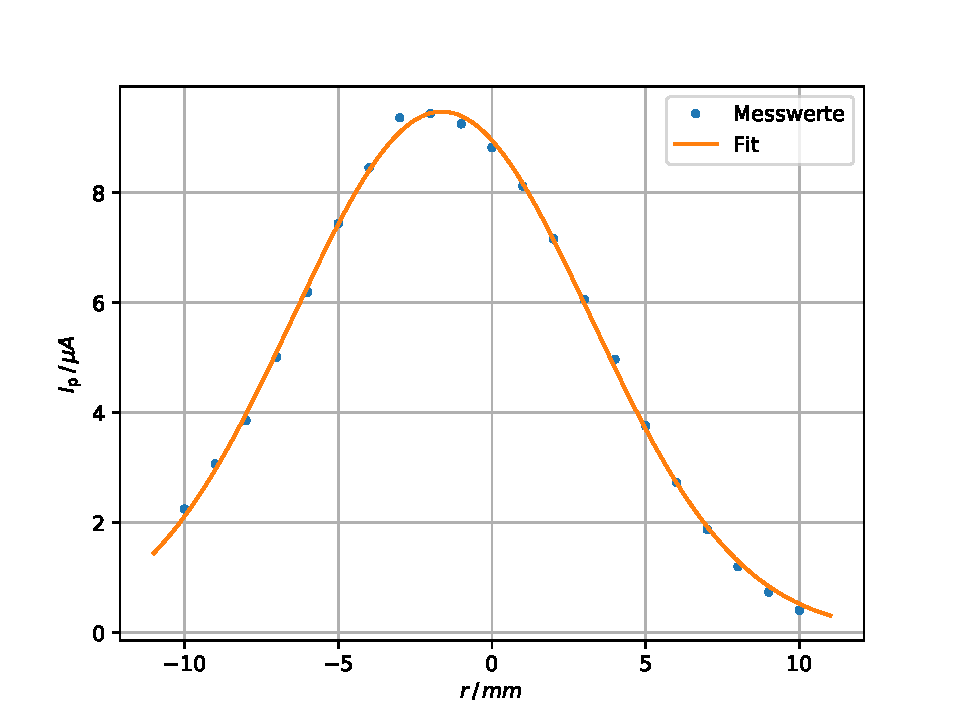
\includegraphics[width=0.7\textwidth]{../Messdaten/plots/T_00.pdf}
  \caption{Plot der in Tabelle \ref{tab: T_00} gelisteten Messwerte. Zusätzlich ist in der Grafik die bestimmte Ausgleichskurve zu sehen.}
  \label{fig: T_00}
\end{figure}
In der Abbildung ist die mit Hilfe von \emph{scipy.optimize} erstelle Fit an die Funktion \eqref{} zu erkennen.
Aus der Ausgleichsrechnung ergeben sich die folgenden Parameter

\begin{align}
  \label{eq: fit_t_00}
  \begin{aligned}
  I_0&=\SI{9.47 \pm 0.05}{\micro\ampere}\\
  d_0&=\SI{-1.63\pm 0.03}{\milli\meter}\\
  \omega&=\SI{9.67\pm0.06}{\per\milli\meter}
\end{aligned}
\end{align}
\FloatBarrier
\subsection{Auswertung der $T_{10}$ Mode}
\FloatBarrier
Die bei der Vermessung der $T_{10}$ Mode aufgenommen Messwerte sind in der Tabelle
\ref{tab: T_10} notiert.
\begin{table} 
\centering 
\caption{Messwerte der T_10 Mode.} 
\label{tab: T_10} 
\begin{tabular}{S S } 
\toprule  
{$r / \si{ \milli\meter }$} & {$I_p / \si{ \micrompere}$} \\ 
\midrule  
-10.0 & 0.2\\ 
-9.0 & 0.5\\ 
-8.0 & 0.8\\ 
-7.0 & 1.3\\ 
-6.0 & 1.6\\ 
-5.0 & 1.9\\ 
-4.0 & 2.0\\ 
-3.0 & 2.0\\ 
-2.0 & 1.5\\ 
-1.0 & 0.8\\ 
0.0 & 0.3\\ 
1.0 & 0.1\\ 
2.0 & 0.0\\ 
3.0 & 0.2\\ 
4.0 & 0.7\\ 
5.0 & 1.2\\ 
6.0 & 1.7\\ 
7.0 & 1.6\\ 
8.0 & 1.3\\ 
9.0 & 1.2\\ 
10.0 & 1.0\\ 
11.0 & 0.6\\ 
12.0 & 0.3\\ 
13.0 & 0.2\\ 
14.0 & 0.1\\ 
15.0 & 0.0\\ 
\bottomrule 
\end{tabular} 
\end{table}
An die Messwerte wurde eine Funktion der Form \eqref{} gefittet, hierbei wird für
die Funktion \emph{curve\_fit} die folgenden Startparameter gewählt
\begin{align*}
  I_{0,1}&=\SI{2.03}{\micro\ampere} & I_{0,2}&=\SI{1.68}{\micro\ampere}\\
  d_{0,1}&=\SI{-4}{\milli\meter}& d_{0,2}&=\SI{6.0}{\milli\meter} \\
  \omega_1&=\SI{1}{\per\milli\meter} &   \omega_2&=\SI{1}{\per\milli\meter}.
\end{align*}
Das Ergebnis der Ausgleichsberechnung lautet
\begin{align}
  \label{eq: fit_t_10}
  \begin{aligned}
  I_{0,1}&=\SI{2.09\pm0.09}{\micro\ampere} & I_{0,2}&=\SI{1.66\pm0.09}{\micro\ampere}\\
  d_{0,1}&=\SI{-4.38\pm0.12}{\milli\meter}& d_{0,2}&=\SI{7.28\pm0.15}{\milli\meter} \\
  \omega_1&=\SI{4.99\pm0.24}{\per\milli\meter} &   \omega_2&=\SI{4.88\pm0.30}{\per\milli\meter}.
\end{aligned}
\end{align}
Die Regressionskurve und die Messdaten sind in Abbildung \ref{fig: T_10} dargestellt.
\begin{figure}[h!]
  \centering
  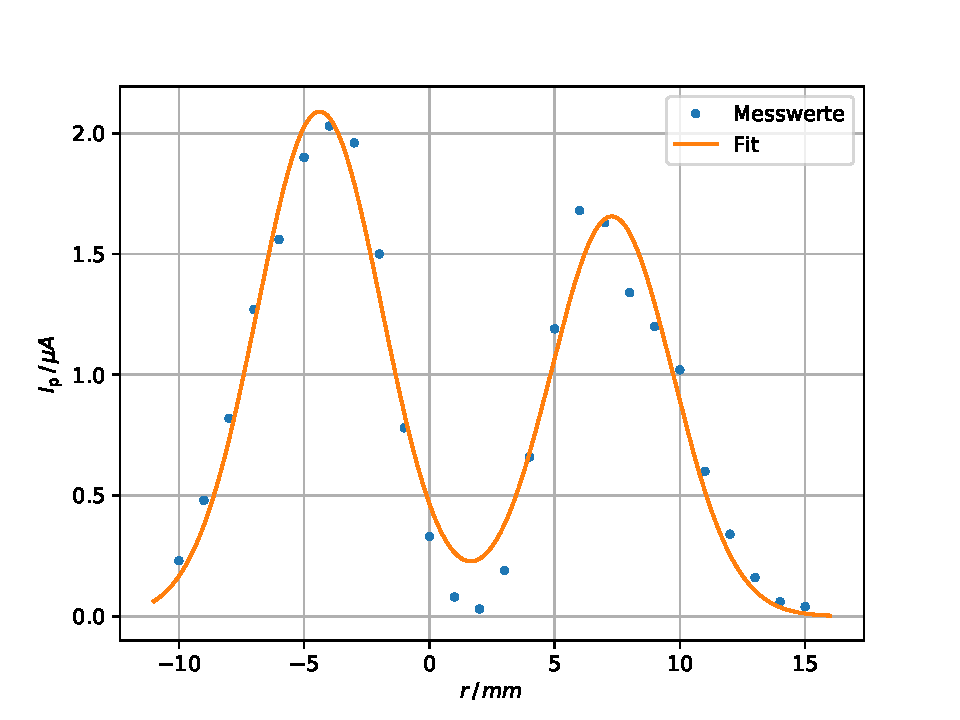
\includegraphics[width=0.8\textwidth]{../Messdaten/plots/T_10.pdf}
  \caption{Plot der in Tabelle \ref{tab: T_10} gelisteten Messwerte. Zusätzlich ist in der Grafik die bestimmte Ausgleichskurve zu sehen.}
  \label{fig: T_10}
\end{figure}
\FloatBarrier
\subsection{Auswertung der Polarisation}

In der Tabelle \ref{tab: pola} sind die notierten Werte der Polarisationsmessung
aufgelistet.
\FloatBarrier
\begin{table} 
\centering 
\caption{Aufgenommene Werte bei der Polarisationsmessungs.} 
\label{tab: pola} 
\begin{tabular}{S S S S S S S S S } 
\toprule  
{$\varphi / \si{ \degree }$} & {$\varphi / \si{ \radian }$} & {$I_p / \si{ \milli\ampere}$} & {$\varphi / \si{ \degree }$} & {$\varphi / \si{ \radian }$} & {$I_p / \si{ \milli\ampere}$} & {$\varphi / \si{ \degree }$} & {$\varphi / \si{ \radian }$} & {$I_p / \si{ \milli\ampere}$} \\ 
\midrule  
0 & 0.00 & 0.36 & 130 & 2.27 & 0.75 & 260 & 4.54 & 0.21\\ 
10 & 0.17 & 0.23 & 140 & 2.44 & 0.74 & 270 & 4.71 & 0.34\\ 
20 & 0.35 & 0.12 & 150 & 2.62 & 0.69 & 280 & 4.89 & 0.47\\ 
30 & 0.52 & 0.04 & 160 & 2.79 & 0.61 & 290 & 5.06 & 0.58\\ 
40 & 0.70 & 0.00 & 170 & 2.97 & 0.51 & 300 & 5.24 & 0.67\\ 
50 & 0.87 & 0.01 & 180 & 3.14 & 0.36 & 310 & 5.41 & 0.74\\ 
60 & 1.05 & 0.06 & 190 & 3.32 & 0.24 & 320 & 5.59 & 0.76\\ 
70 & 1.22 & 0.16 & 200 & 3.49 & 0.14 & 330 & 5.76 & 0.73\\ 
80 & 1.40 & 0.28 & 210 & 3.67 & 0.06 & 340 & 5.93 & 0.64\\ 
90 & 1.57 & 0.41 & 220 & 3.84 & 0.01 & 350 & 6.11 & 0.52\\ 
100 & 1.75 & 0.50 & 230 & 4.01 & 0.00 & 360 & 6.28 & 0.39\\ 
110 & 1.92 & 0.62 & 240 & 4.19 & 0.03 &  &  & \\ 
120 & 2.09 & 0.71 & 250 & 4.36 & 0.10 &  & & \\ 
\bottomrule 
\end{tabular} 
\end{table}

An die Messwerte wird die Funktion

\begin{equation}
  \label{eq: func_polarisation}
  I(\phi)=I_0\sin^2\left(\phi-\phi_0\right)
\end{equation}
mit den folgenden Parametern gefittet:

\begin{align}
  \label{eq: fit_pola}
  \begin{aligned}
  I_0&=\SI{0.748\pm0.005}{\milli\ampere}\\
  \phi_0&=\SI{0.792\pm0.006}{\radian}
\end{aligned}
\end{align}
Die Messwerte und die Ausgleichskurve sind in Abbildung \ref{fig: pola} skizziert.

\begin{figure}[h!]
  \centering
  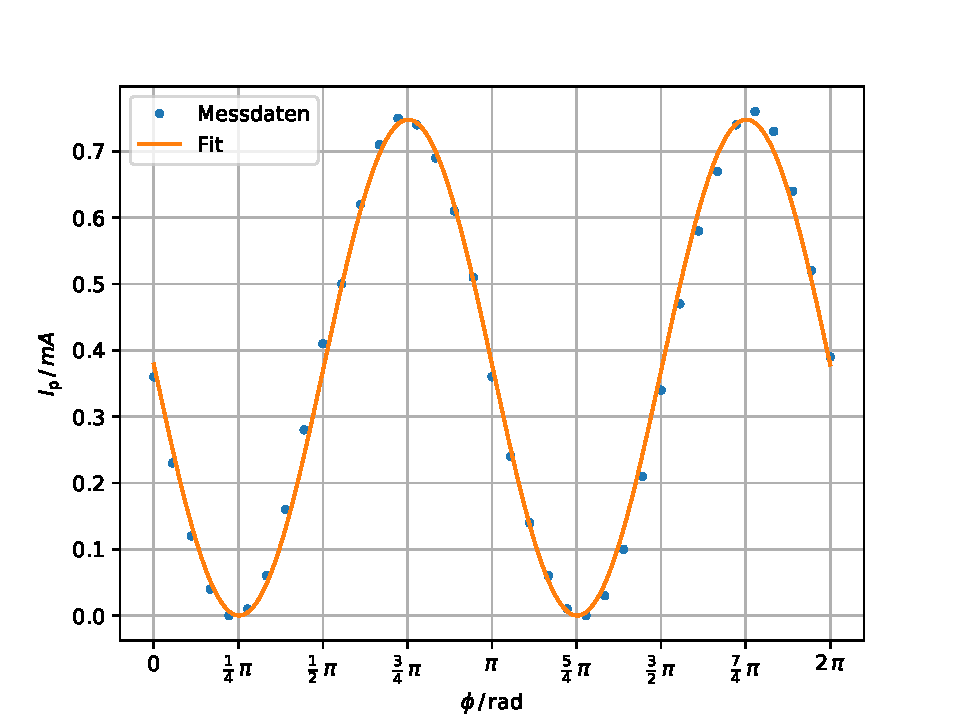
\includegraphics[width=0.8\textwidth]{../Messdaten/plots/pola.pdf}
  \caption{Plot der in Tabelle \ref{tab: pola} gelisteten Messwerte. Zusätzlich ist in der Grafik die bestimmte Ausgleichskurve zu sehen.}
  \label{fig: pola}
\end{figure}
\FloatBarrier

\FloatBarrier
\subsection{Wellenlängenbestimmung}
Die Messwerte, um die Wellenlänge des Lasers zu bestimmen, befinden sich in Tabelle  \ref{tab: wellenlaenge}.
Bei der Messung betrug der Abstand zum Schirm $l=\SI{83}{\centi\meter}$
und wurde mit einem Gitter mit dem Gitterabstand von $a=\SI{1e-5}{\meter}$ durchgeführt.
\begin{table} 
\centering 
\caption{Aufgenommene Messwerte für die Wellenlängenbestimmung. Der Winkel $	\theta$ und die Wellenlänge $\lambda$ werden mit den Gleichung \eqref{} und \eqref{} bestimmt. Der Abstand zum Schirm beträgt $l=\SI{83}{\centi\meter}$ und der Gitterabstand $a=\SI{1e-5}{\meter}$.} 
\label{tab: wellenlaenge} 
\begin{tabular}{S S S S } 
\toprule  
{$n $} & {$d / \si{ \centi\meter}$} & {$\theta / \si{ \radian}$} & {$\lambda / \si{ \nano\meter}$} \\ 
\midrule  
1.0 & 10.8 & 0.1 & 649.2\\ 
2.0 & 21.6 & 0.1 & 645.2\\ 
3.0 & 32.7 & 0.2 & 644.2\\ 
4.0 & 44.0 & 0.3 & 640.5\\ 
5.0 & 51.2 & 0.3 & 589.5\\ 
6.0 & 70.0 & 0.4 & 647.6\\ 
\bottomrule 
\end{tabular} 
\end{table}

In der Tabelle werden außerdem die für jede Ordnung $n$ errechneten Wellenlängen $\lambda$ und Winkel $\theta$
mit aufgelistet. Hierbei wird die Wellenlänge mit Formel \eqref{} und der Winkel mit \eqref{} berechnet.
Über alle vermessenen Ordnungen gemittelt ergibt sich für die Wellenlänge
\begin{equation}
  \label{eq: mittelwert_wellenlaenge}
  \ov{\lambda}=\SI{636\pm9}{\nano\meter}.
\end{equation}
\FloatBarrier
\FloatBarrier
\subsection{Untersuchugn der Stabilitätsbedingung}
Die Stabilitätsbedingung wird für zwei verschiedene Konfigurationen untersucht,
zum einen werden für den Resonator zwei konkave Spiegel verwendet und zum andern
ein konkaver und ein flacher Spiegel.
Um einen Vergleich zwischen den Messwerten und der Theorie zu ermöglichen, wird der gemessene
Photostrom $i_p$ wie folgt umkskaliert:
\begin{equation*}
  I_p \rightarrow \frac{I_p\cdot c}{I_{p,max}}.
\end{equation*}
Hierbei wird der Skalierungsfaktor  $c$ aus Startlänge $d_0$ der jeweiligen Konfiguration (legt $r_i$ fest) und der Formel
\eqref{} berechnet.
\begin{equation*}
  c=g_1g_2(d_0, r_1, r_2)
\end{equation*}

\FloatBarrier
\FloatBarrier
\subsubsection{Konkav-Konkave Konfiguration}

Die für diese Konfiguration aufgenommenen Messwerte befinden sich in Tabelle \ref{fig: konkon}.
\begin{table} 
\centering 
\caption{Aufgenommene Messwerte für die Untersuchung der Stabilitätsbedingung bei Konkav-Konkave Konfiguration. Der Umskalierungsfaktor $c$ beträgt $\num{0.12}$.} 
\label{tab: konkon} 
\begin{tabular}{S S S } 
\toprule  
{$ d / \si{ \centi\meter}$} & {$ I_p / \si{ \milli\ampere}$} & {$ \frac{I_p\cdot c}{I_{p,max}} $} \\ 
\midrule  
91 & 0.43 & 0.12\\ 
100 & 0.40 & 0.11\\ 
106 & 0.42 & 0.12\\ 
116 & 0.33 & 0.09\\ 
126 & 0.35 & 0.10\\ 
131 & 0.37 & 0.11\\ 
134 & 0.24 & 0.07\\ 
141 & 0.34 & 0.10\\ 
147 & 0.16 & 0.05\\ 
157 & 0.42 & 0.12\\ 
\bottomrule 
\end{tabular} 
\end{table}

Der Skalierungsfaktor trägt den Wert $c=\num{0.12}$.
An die skalierten Messwerte wird eine quadratische Funktion der Form
\begin{equation*}
  f(d)=a\,d^2+b\,d+c
\end{equation*}
gefittet. Aus der Ausgleichsrechnung folgen die Werte
\begin{align}
  \label{eq: fit_konkon}
  \begin{aligned}
    a&=\SI{2.0\pm 1.9 e-5}{\per\square\milli\meter}\\
    b&=\SI{-6\pm5 e-3}{\per\milli\meter}\\
    c&=\num{0.47\pm0.28}.
  \end{aligned}
\end{align}
In der Grafik \ref{fig: konkon} werden die Messwerte, der Fit und die Theoriekurve \eqref{} miteinander verglichen.

\begin{figure}[h!]
  \centering
  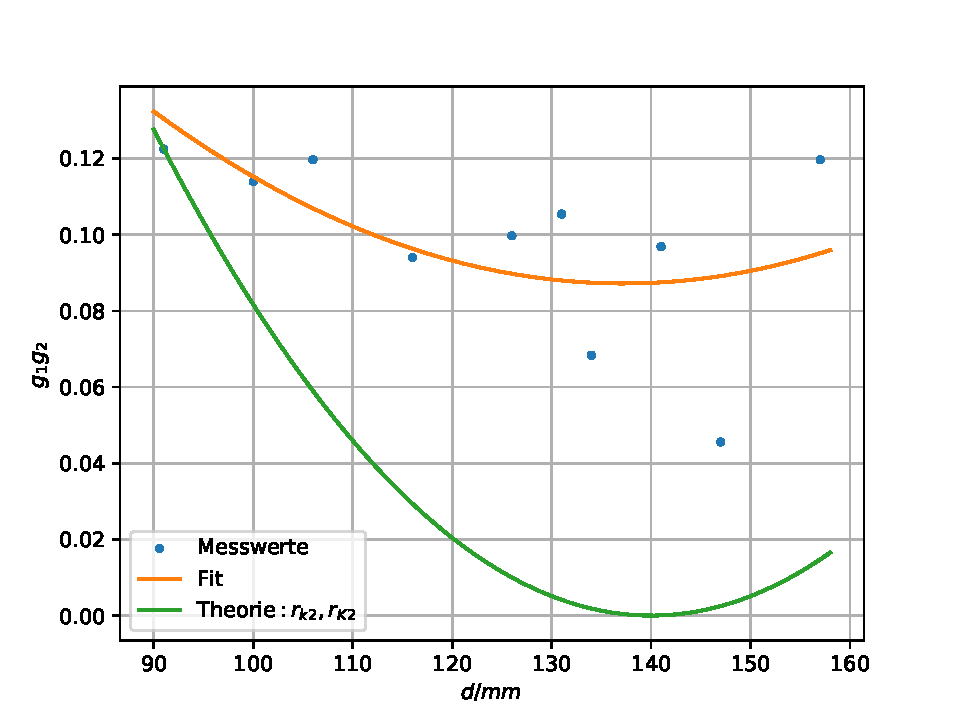
\includegraphics[width=0.8\textwidth]{../Messdaten/plots/konkon.pdf}
  \caption{Plot der in Tabelle \ref{tab: konkon} gelisteten Messwerte. Zusätzlich ist in der Grafik die bestimmte Ausgleichskurve und die Theoriekurve \eqref{} zu sehen.}
  \label{fig: konkon}
\end{figure}

\FloatBarrier
\FloatBarrier
\subsubsection{Konkav-Flache Konfiguration}
Die Messwerte sind in Tabelle \ref{tab: konflach} aufgelistet.
Eine Skalierung erfolgt mit dem Faktor $c=\num{0.46}$
\begin{table} 
\centering 
\caption{Aufgenommene Messwerte für die Untersuchung der Stabilitätsbedingung bei Konkav-Flache Konfiguration. Der Umskalierungsfaktor $c$ beträgt $\num{0.46}$.} 
\label{tab: konflach} 
\begin{tabular}{S S S } 
\toprule  
{$ d / \si{ \centi\meter}$} & {$ I_p / \si{ \milli\ampere}$} & {$ \frac{I_p\cdot c}{I_{p,max}}$} \\ 
\midrule  
75 & 0.15 & 0.46\\ 
82 & 0.13 & 0.40\\ 
87 & 0.11 & 0.34\\ 
94 & 0.10 & 0.31\\ 
99 & 0.09 & 0.28\\ 
106 & 0.00 & 0.00\\ 
\bottomrule 
\end{tabular} 
\end{table}

An die Messwerte wird eine Gerade
\begin{equation*}
  g(d)=md+a
\end{equation*}
gefittet. Die Parameter $m$ und $a$ werden mittels Regressionsberechnung zu
\begin{align}
  \label{eq: konflach}
  \begin{aligned}
    m&=\SI{1.29 \pm 0.29 e-2}{\per\milli\meter}\\
    a&=\num{1.46\pm0.27}.
  \end{aligned}
\end{align}
Die Regressionskurve wird mit den Messwerten und der Theoriekurve \eqref{} in Abbildung \ref{fig: konflach} dargestellt.

\begin{figure}[h!]
  \centering
  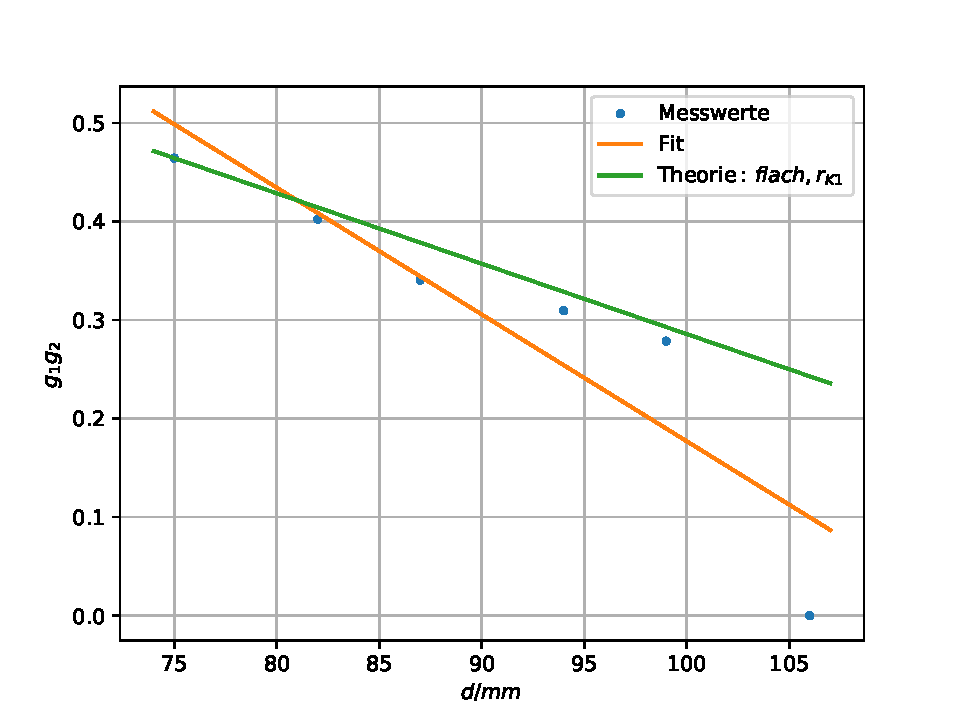
\includegraphics[width=0.8\textwidth]{../Messdaten/plots/konflach.pdf}
  \caption{Plot der in Tabelle \ref{tab: konflach} gelisteten Messwerte. Zusätzlich ist in der Grafik die bestimmte Ausgleichsgerade und die Theoriekurve \eqref{} zu sehen.}
  \label{fig: konflach}
\end{figure}
\FloatBarrier

\section{Diskussion}
Im Folgenden sollen die Ergebnisse der Messungen interpretiert und in Beziehung zur Präzision des verwendeten Aufbaus gestellt werden. \\
Zunächst zur Messung der Maße der verwendeten Proben. Hier war eine präzise Messung aufgrund der deformierten Proben nur sehr schwer möglich.
Da die Proben fest auf den Kunststoffplatten befestigt sind, konnte insbesondere die Dicke der Zinkprobe mit dem Messschieber nur sehr ungenau aufgenommen werden.
Ungenauigkeiten an dieser Stelle des Versuches haben immense Auswirkungen auf die Bestimmung der mikroskopischen Größen. Etwa die Teilchenzahl pro Volumen
ist direkt Abhängig von der Dicke $d$ [siehe \eqref{eq:steig_teil_anz_konstb}]. In der Literatur \cite{dem2} findet man für den spezifischen Widerstand von Kupfer den Wert $\SI{0.017}{\ohm \milli \meter^2 \per \meter}$. Der Vergleich %cite, a?
mit dem gefundenen Wert \eqref{eq: res_spez_widerstand} (Abweichung im Mittel $630\%$) bestätigt exemplarisch die nur sehr ungenaue Bestimmung der mikroskopischen Größen. %Abweichung im Mittel
Darüber hinaus bildet die Berechnung der Magnetfeldstärke aus dem anfangs ermittleten Zusammenhang zum Spulenstrom \eqref{eq: hysterese} eine weitere Quelle systematischer
Fehler. Das Netzgerät zeigte im Laufe der Messung sehr häufig technische Probleme auf, was auf eine Überhitzung zurück zu führen ist. \\
Davon abgesehen ermöglicht der Aufbau eine relativ genaue Bestimmung der Hallspannung, wie sich besonders bei der Versuchsereihe mit der Kupferprobe zeigt. Die Annäherung
an einen linearen Zusammenhang zwischen Spulenstrom und Hallspannung \eqref{eq: steigung_konst_I} gelingt hier mit großer Präzision. Weiterhin zeigt sich, dass die jeweiligen
Ergebnisse aus der Messung mit konstantem Spulenstrom bzw. konstantem Querstrom nur geringfügig voneinander abweichen. Dies zeigt, dass der Aufbau im Rahmen der erwähnten
Ungenauigkeiten relativ aussagekräftige Ergenisse liefert.\\
Ausgehend von der Annahme, dass Kupfer ein Elektronenleiter ist,
kann aufgrund des Vorzeichens der Hallspannung geschlossen werden, dass es sich bei Zink um einen Ionen- bzw. Lochleiter handelt. \\


\printbibliography
\newpage
\section{Anhang}
\begin{figure}
  \centering
  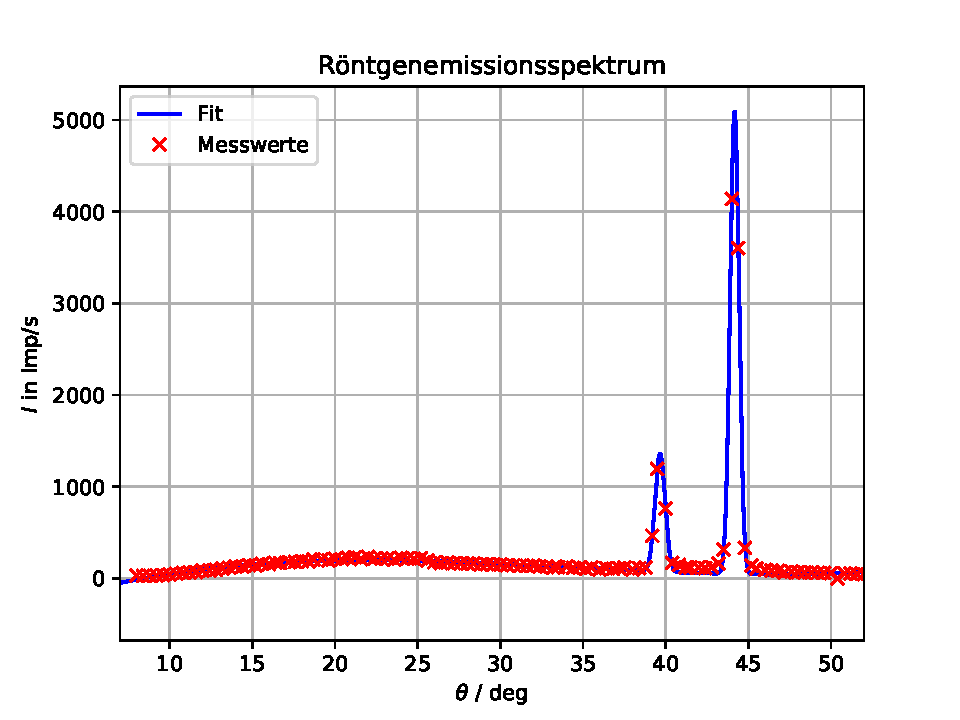
\includegraphics[width = \textwidth]{pics/schokolade.pdf}
  \caption{Fit an Daten des Röngenemissionsspektrums. Hierbei wird das kontinuierliche Bremsspektrum durch ein Polynom
  dritten Grades dargestellt und die beiden Peaks des charakteristischen Spektrums durch eine summierte Gaußfunktion. Das Gesamte
  Spektrum ergibt sich aus der Summe der beiden Spektren.}
  \label{fig: fit_emissionsspektrum}
\end{figure}
Für den linken Peak ergeben sich Mittelwert $x\ua{0, 1}$ und Standardabweichung $\sigma\ua{1}$ zu
\begin{align}
  x\ua{0, 1} &= \SI{9.073(2)}{\kilo\eV} & \sigma\ua{1} &= \SI{66(2)}{\eV}.
\intertext{Entsprechend für den rechten Peak}
  x\ua{0, 2} &= \SI{8.1861(4)}{\kilo\eV} & \sigma\ua{2} &= \SI{47.8(7)}{\eV}.
\end{align}

\end{document}
